% ---------- Datei: chapters/06_uebergabe_und_betrieb.tex ----------
\chapter{Übergabe und Betrieb}

\section{Monitoring}
Das Tool \textit{Network Topology} im Google Cloud Network Intelligence Center hat die hybride Hub-and-Spoke-Struktur erfolgreich überwacht und visualisiert.

\begin{figure}[!ht]
\centering
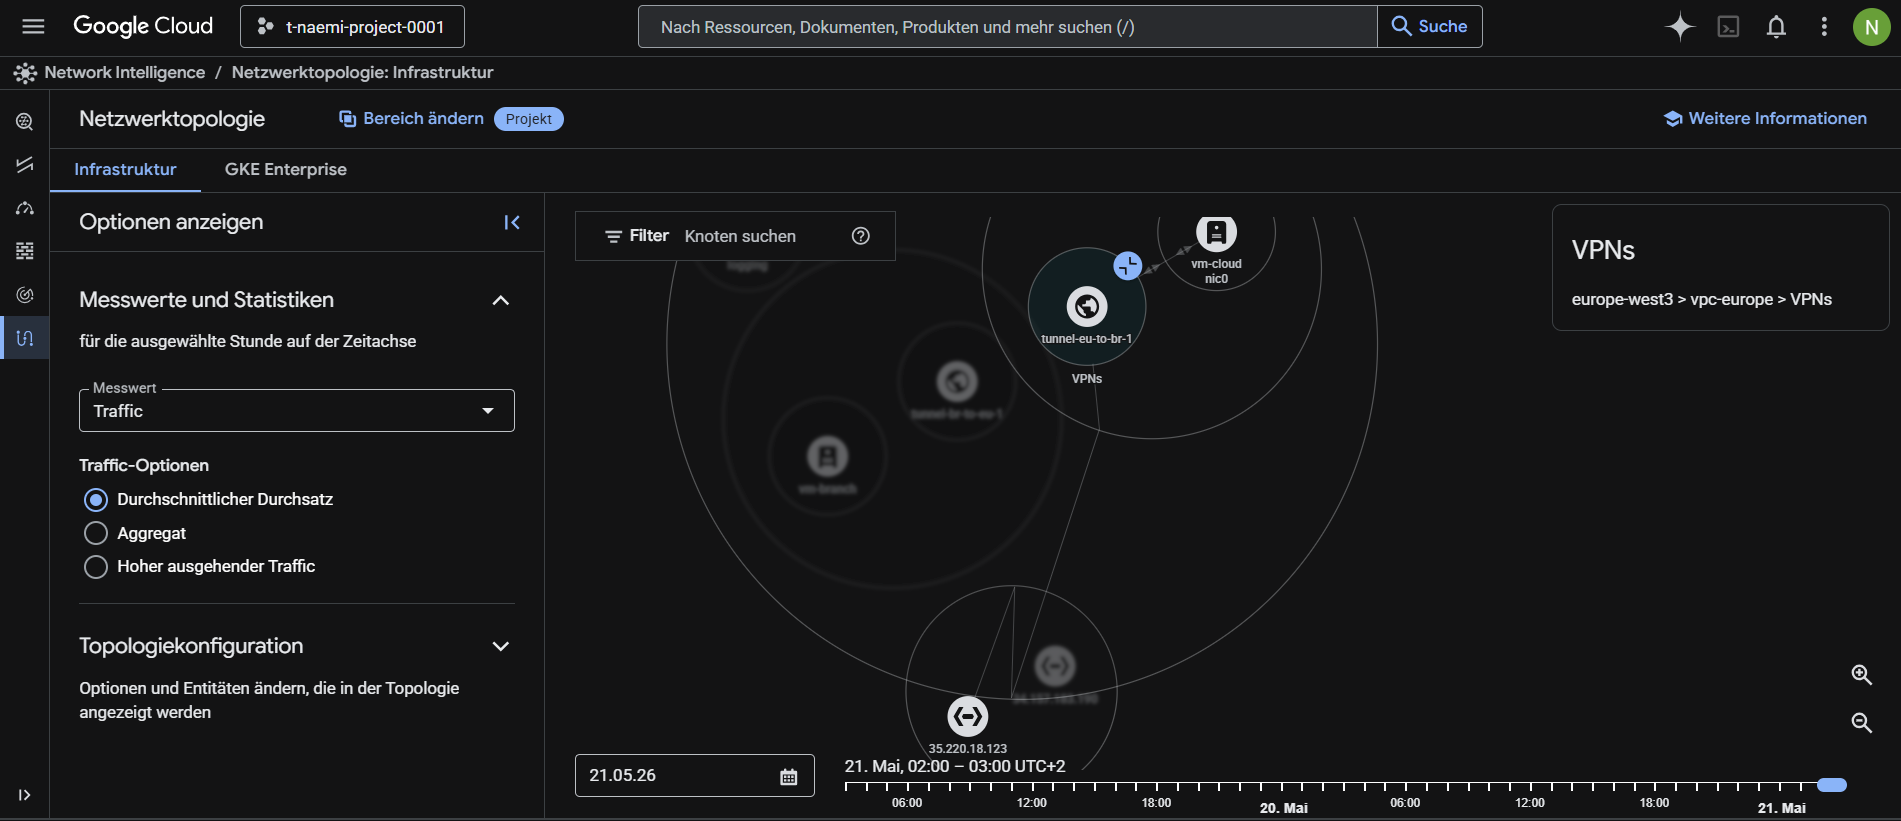
\includegraphics[width=\textwidth]{images/Monitoring.png}
\caption{Netzwerktopologie in Google Network Intelligence Center}
\label{fig:monitoring}
\end{figure}

\section{Übergabe und Cleanup}
Nach der Projektübergabe inklusive Dokumentation und technischer Einweisung hat das Team alle temporären Test-Ressourcen zur Vermeidung unnötiger Cloud-Kosten manuell entfernt (Teardown).

\begin{figure}[!ht]
\centering
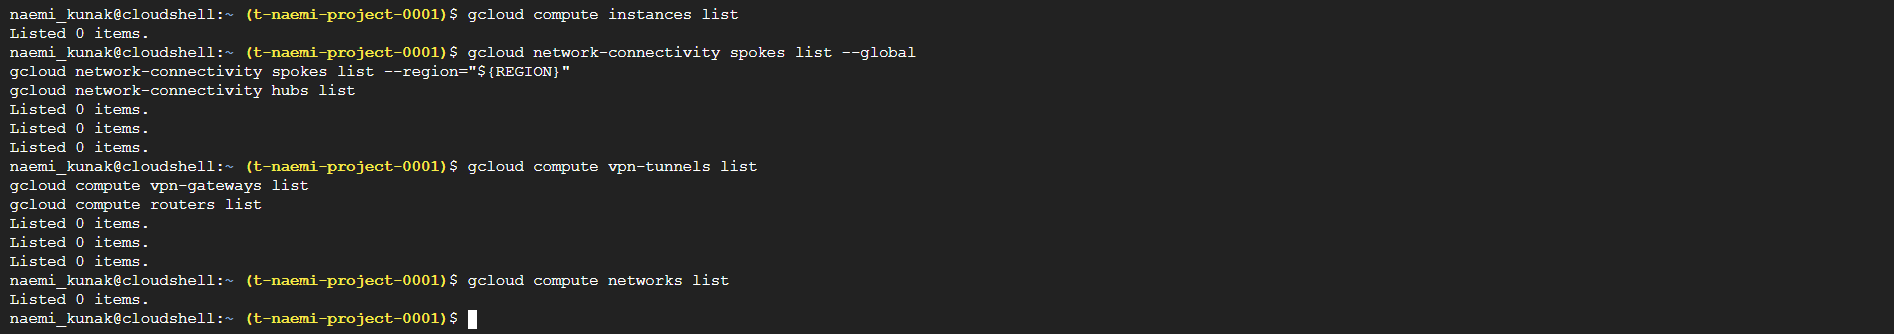
\includegraphics[width=\textwidth]{images/Clean-up.png}
\caption{Überprüfung des Teardowns}
\label{fig:cleanup}
\end{figure}